\documentclass[11pt,a4paper]{article}
\usepackage[T1]{fontenc}
\usepackage[margin=2.3cm]{geometry}
\usepackage{amsmath,amssymb}
\usepackage{graphicx}
\usepackage[dvipsnames]{xcolor}
\usepackage{enumitem}
\usepackage[colorlinks=true,linkcolor=blue,urlcolor=blue]{hyperref}
\setlength{\parskip}{0.6em}
\setlength{\parindent}{0pt}
\begin{document}

\begin{center}{\LARGE\bfseries openbatterycell}\\[0.4em]{\large Build and size an electrochemical cell for a target voltage, in three sessions.}\\[0.2em]\small PAN IIT OSS explainer \textbullet{} secondary school to diploma / undergraduate (levels 3-5)\end{center}

\section*{Why this exists}
A battery cell turns the chemical difference between two metals into an electric voltage. This explainer follows the cell from a lemon to a simulation: electrode potentials, series and parallel packs, Faraday's law and the Nernst equation, using only arithmetic and a little calculus.

\section*{The end goal}
Build and size an electrochemical cell for a target voltage. The end goal is to build and size an electrochemical cell for a target voltage and to understand how it behaves as it is used: voltage, capacity, internal resistance, power and heat. The same ideas underlie every battery from a torch cell to a grid store, but this is an educational model, not a design tool, and real lithium and lead-acid batteries can be dangerous.

\section*{How the three sessions build up}
\begin{enumerate}[nosep]
\item \textbf{Session 1: Two metals make a cell} (Level 1, conceptual interactive model, 60 min).
\item \textbf{Session 2: Voltage, capacity and Faraday's law} (Level 2, mathematical engineering model, 75 min).
\item \textbf{Session 3: A cell that runs down} (Level 3, simulation and validation, 90 min).
\end{enumerate}

\section{Session 1: Two metals make a cell}

\subsection*{A. Real-world problem}
Push a zinc nail and a copper coin into a lemon and connect them to a small meter: it shows a voltage, although nothing was plugged in. A torch battery is the same idea in a tidier box. Where does the voltage come from, which way do the electrons go, and how do you stack several cells to reach the voltage a device needs? (Real lithium and lead-acid batteries can be dangerous; this repo is an educational model, not a how-to for building them.)

\subsection*{B. Concept and theory}
Some metals give up electrons more easily than others. Chemists rank them with the standard electrode potential E0 in volts, measured against the standard hydrogen electrode, which is defined as 0 V. The more negative the number, the more eagerly the metal gives up electrons. When two metals are joined by a wire and a salt bridge, the metal lower on the ladder is the anode and pushes electrons into the wire; the metal higher on the ladder is the cathode and receives them. The cell voltage is the height difference E = E(cathode) - E(anode). In the solution, anode metal dissolves as positive ions and positive ions at the cathode take electrons and become metal; the salt bridge lets charged ions drift so neither beaker builds up charge. Cells connected in series add their voltages.

\begin{itemize}[nosep]
\item E0: standard electrode potential of a metal (reduction, 25 C, 1 mol/L) (V)
\item E\_cell: cell voltage = E0(cathode) - E0(anode) (V)
\item n: number of identical cells in series (no unit)
\item V\_total: voltage of the stack, n times E\_cell (V)
\end{itemize}

\begin{equation*}
E_{cell}=E^{0}_{cathode}-E^{0}_{anode}
\end{equation*}

\begin{equation*}
\text{Zn/Cu (Daniell): } E_{cell}=0.34-(-0.76)=1.10\ \mathrm{V}
\end{equation*}

\begin{equation*}
V_{total}=n\,E_{cell},\qquad n=\left\lceil \frac{V_{target}}{E_{cell}}\right\rceil
\end{equation*}

\begin{center}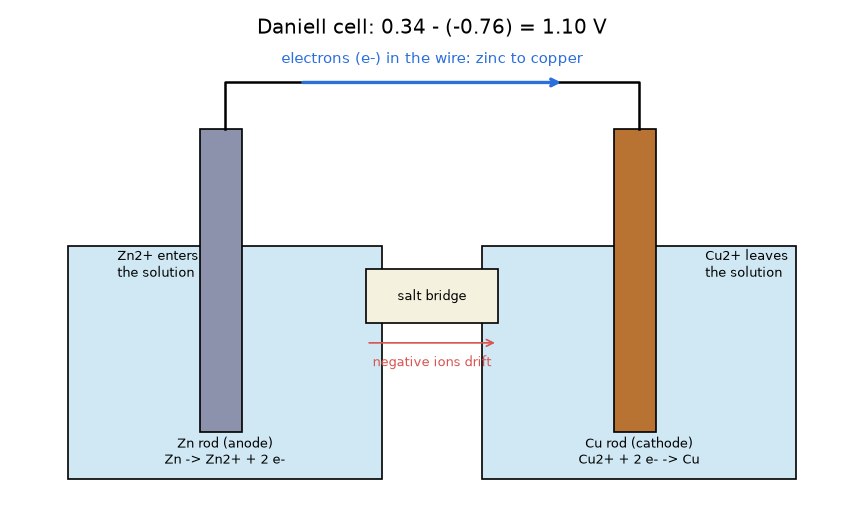
\includegraphics[width=0.85\linewidth]{figures/s01_cell_picture.png}\\\small A Daniell cell: electrons in the wire from zinc to copper, ions in the solution and salt bridge, 1.10 V.\end{center}

\subsection*{E. Worked example}
A toy needs at least 4.5 V. How many zinc-copper cells in series are needed, and what voltage do they give?
\begin{enumerate}[nosep]
\item One zinc-copper cell: E = 0.34 - (-0.76) = 1.10 V.
\item Cells needed: 4.5 / 1.10 = 4.09, and we cannot build 0.09 of a cell, so round up to 5.
\item Total: 5 x 1.10 = 5.50 V, which is at least 4.5 V.
\item Check: 4 cells would give only 4.40 V, which is too low.
\end{enumerate}
\textbf{Answer.} 5 cells in series, 5.50 V.

\subsection*{F. Questions}
\begin{enumerate}[nosep]
\item \textbf{Conceptual.} In a zinc-copper cell, why do the electrons travel from the zinc to the copper, and what stops the current if you remove the salt bridge?
\item \textbf{Numerical.} An iron-silver cell is built (iron anode, silver cathode). Find the cell voltage and the number of cells in series needed for 5 V.
\item \textbf{Graph and simulation interpretation.} In the stack graph, the line for a zinc-copper cell and the line for an iron-copper cell (0.34 - (-0.44) = 0.78 V) both start at zero. Which line is steeper and what does the slope mean? Which stack reaches 3 V with fewer cells?
\item \textbf{Design and optimisation challenge.} Design: a small radio needs at least 6 V from water-based cells made from the metals zinc, iron, copper and silver. Choose the pair that needs the fewest cells and the pair you would choose if silver is too expensive. Why is lithium not an option here?
\end{enumerate}

\section{Session 2: Voltage, capacity and Faraday's law}

\subsection*{A. Real-world problem}
You want a 12 V, 2 Ah supply for a small light and you have only 1.10 V cells that each hold 1 Ah. How many cells, connected how? And how many grams of zinc must be inside, at the very least? A designer answers these before building anything, and the same arithmetic scales from a torch to a battery pack. (Educational model of ideal cells: real lithium and lead-acid packs can burn if shorted, overheated or overcharged.)

\subsection*{B. Concept and theory}
Series connection: voltages add and the capacity is that of one cell. Parallel connection: voltage stays and capacities add. A pack with ns cells in each string and npar strings has V = ns V\_cell, capacity Q = npar Ah\_cell, and stores energy W = V x Q in watt-hours. Charge: one ampere-hour is 3600 coulombs. One mole of electrons carries F = 96485 coulombs, and each zinc atom gives up n = 2 electrons, so Q coulombs dissolve Q / (n F) moles of zinc, i.e. a mass m = Q M / (n F) with M = 65.38 g/mol. For one ampere-hour that is 1.2197 g of zinc. Because every series cell passes the same charge, the total zinc in a pack is (series cells) x (pack Ah) x 1.2197 g per Ah.

\begin{itemize}[nosep]
\item V\_cell: voltage of one cell (Zn/Cu, ideal) (V)
\item ns, npar: cells in series per string, number of strings in parallel (no unit)
\item Ah\_cell: capacity of one cell (Ah)
\item Q: charge that flows (C (1 Ah = 3600 C))
\item F: Faraday constant, charge of one mole of electrons (96485 C/mol)
\item n: electrons per metal ion (2 for Zn2+) (no unit)
\item M: molar mass of the metal (65.38 for zinc) (g/mol)
\item m: mass of metal consumed (g)
\item W: energy W = V x Ah (Wh)
\end{itemize}

\begin{equation*}
V_{pack}=n_s V_{cell},\quad Q_{pack}=n_p\,Ah_{cell},\quad W=V_{pack}Q_{pack}\ \ (\mathrm{Wh})
\end{equation*}

\begin{equation*}
Q\,[\mathrm{C}]=3600\times Ah,\qquad \text{moles of electrons}=Q/F
\end{equation*}

\begin{equation*}
m=\frac{Q\,M}{n\,F}\qquad\Rightarrow\qquad m_{Zn}=\frac{3600\times 65.38}{2\times 96485}=1.2197\ \mathrm{g\ per\ Ah}
\end{equation*}

\begin{equation*}
n_s=\left\lceil \frac{V_{target}}{V_{cell}}\right\rceil,\qquad n_p=\left\lceil \frac{Ah_{target}}{Ah_{cell}}\right\rceil
\end{equation*}

\begin{center}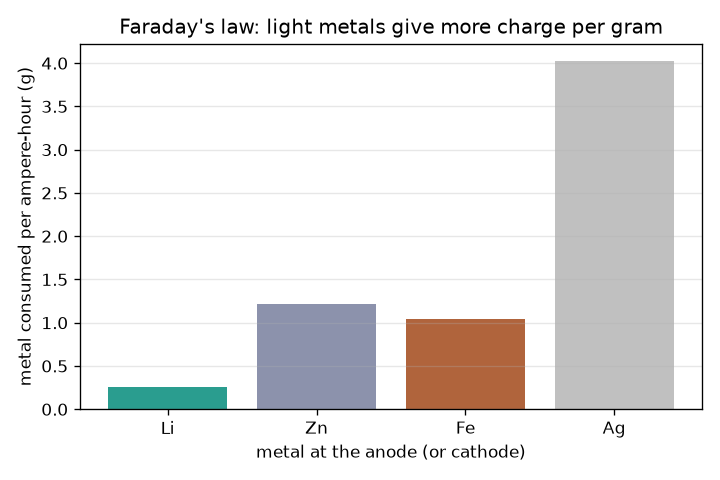
\includegraphics[width=0.85\linewidth]{figures/s02_mass_per_ah.png}\\\small Grams of metal consumed per ampere-hour from Faraday's law: lithium 0.259, zinc 1.220, iron 1.042, silver 4.025.\end{center}

\subsection*{E. Worked example}
Design a pack of at least 12 V and at least 2 Ah from 1.10 V, 1 Ah zinc-copper cells. Give the cell count, the energy and the minimum zinc mass.
\begin{enumerate}[nosep]
\item Series: 12 / 1.10 = 10.9, round up: ns = 11 cells, V = 11 x 1.10 = 12.1 V.
\item Parallel: 2 / 1 = 2 strings, so the capacity is 2 x 1 = 2 Ah.
\item Total cells = 11 x 2 = 22. Energy W = 12.1 V x 2 Ah = 24.2 Wh (check: 22 cells x 1.10 V x 1 Ah = 24.2 Wh).
\item Zinc per cell for 1 Ah: Q = 3600 C, m = 3600 x 65.38 / (2 x 96485) = 1.2197 g.
\item Zinc in the pack: 22 x 1.2197 = 26.8 g (at least; real cells need extra for losses).
\end{enumerate}
\textbf{Answer.} 11 cells in series x 2 strings = 22 cells, 12.1 V, 2 Ah, 24.2 Wh, at least 26.8 g of zinc.

\subsection*{F. Questions}
\begin{enumerate}[nosep]
\item \textbf{Conceptual.} Why does connecting cells in parallel not raise the voltage, and why does connecting cells in series not increase how long a light runs?
\item \textbf{Numerical.} How much zinc is consumed by a 0.5 A current flowing for 4 hours? How many ampere-hours is that?
\item \textbf{Graph and simulation interpretation.} On the zinc graph for 11 cells in series, read the zinc mass for a pack capacity of 2 Ah. How would the line change if you used 5 series cells instead, and why is the line straight?
\item \textbf{Design and optimisation challenge.} Design: a pack must give at least 6 V and 3 Ah from 1.10 V cells that each hold only 0.8 Ah. Find ns and np, the energy, and the zinc mass. State one reason you might accept a pack with more cells.
\end{enumerate}

\section{Session 3: A cell that runs down}

\subsection*{A. Real-world problem}
A torch cell does not stay at its printed voltage: it sags when the torch is bright, recovers when it is dimmed, fades when cold and, if shorted, gets hot fast. Why? Three effects explain it: the chemicals are used up (Nernst), the cell has an internal resistance, and heat is made wherever current flows through that resistance. Can you simulate them with one small model and check it against Faraday's law? (Real lithium and lead-acid batteries can be dangerous; every parameter here is illustrative and the model is educational only.)

\subsection*{B. Concept and theory}
Nernst equation: for Zn + Cu2+ -\textgreater{} Zn2+ + Cu with reaction quotient Q = [Zn2+] / [Cu2+], E = E0 - (R T / (n F)) ln Q, with n = 2. At 25 C, R T / F = 25.69 mV, so each factor e in Q changes E by 25.69 mV / n; each decade (factor 10) changes E by 2.303 R T / (n F), i.e. 59.16 mV for n = 1 and 29.58 mV for the Daniell cell. Discharge: drawing charge q reacts q / (n F) moles, which lowers [Cu2+] and raises [Zn2+] in a solution of volume V\_sol. With internal resistance r and load R, I = E / (R + r) and the terminal voltage is V = E - I r. Delivered power is P = I\textasciicircum{}2 R = E\textasciicircum{}2 R / (R + r)\textasciicircum{}2, maximal at R = r where P\_max = E\textasciicircum{}2 / (4 r) and efficiency R / (R + r) is 50 percent. A short circuit (R near 0) gives I = E / r and heat I\textasciicircum{}2 r, warming the cell by the lumped model C\_th dT/dt = I\textasciicircum{}2 r - hA (T - T\_amb). Illustrative extras: r rises as Cu2+ runs out and falls as temperature rises.

\begin{itemize}[nosep]
\item E0: standard cell voltage (1.10 V for Zn/Cu) (V)
\item Q: reaction quotient [Zn2+] / [Cu2+] (no unit)
\item R, T: gas constant 8.314 J/(mol K), absolute temperature (J/(mol K), K)
\item n, F: electrons transferred (2), Faraday constant (no unit, C/mol)
\item q: charge drawn so far (C)
\item r: internal resistance of the cell (0.8 ohm at 25 C, illustrative) (ohm)
\item R\_load: resistance of the load (ohm)
\item I, V: current and terminal voltage (A, V)
\item C\_th, hA: heat capacity of the cell (40 J/K) and heat loss coefficient (0.15 W/K), illustrative (J/K, W/K)
\end{itemize}

\begin{equation*}
E=E^{0}-\frac{RT}{nF}\ln Q,\qquad Q=\frac{[\mathrm{Zn^{2+}}]}{[\mathrm{Cu^{2+}}]}
\end{equation*}

\begin{equation*}
\Delta E_{\text{decade}}=\frac{2.303\,RT}{nF}=29.58\ \mathrm{mV}\ (n=2),\ 59.16\ \mathrm{mV}\ (n=1)\ \text{at 25 C}
\end{equation*}

\begin{equation*}
I=\frac{E}{R_{load}+r},\qquad V=E-Ir,\qquad \frac{dq}{dt}=I(q)
\end{equation*}

\begin{equation*}
P=\frac{E^{2}R_{load}}{(R_{load}+r)^{2}},\quad P_{max}=\frac{E^{2}}{4r}\ \text{at}\ R_{load}=r,\quad \eta=\frac{R_{load}}{R_{load}+r}
\end{equation*}

\begin{equation*}
C_{th}\frac{dT}{dt}=I^{2}r-hA\,(T-T_{amb}),\qquad I=\frac{E}{r}\ \text{for a short}
\end{equation*}

\begin{center}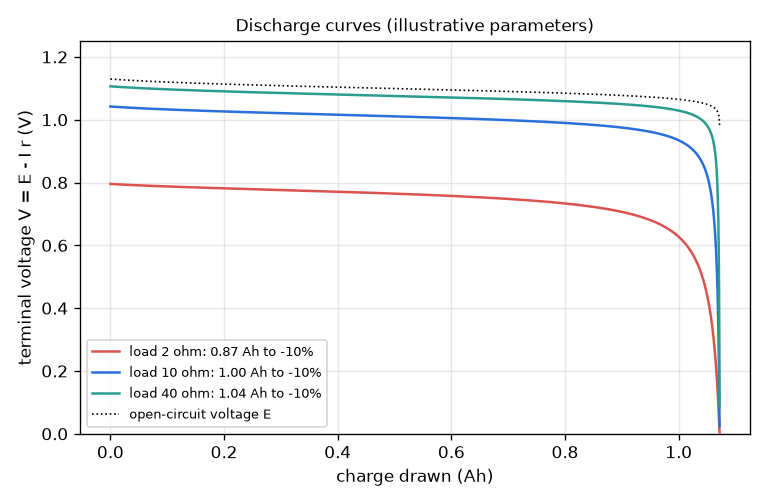
\includegraphics[width=0.85\linewidth]{figures/s03_discharge_curve.png}\\\small Discharge curves for 2, 10 and 40 ohm loads (illustrative parameters), with the open-circuit voltage dotted.\end{center}

\subsection*{E. Worked example}
A Daniell cell starts with [Zn2+] = 0.10 mol/L and [Cu2+] = 1.0 mol/L at 25 C. Find its voltage, then the current, terminal voltage and powers when it drives a 10 ohm load (internal resistance 0.8 ohm, plus 0.05 x 0.8 from the depletion term at the start).
\begin{enumerate}[nosep]
\item Q = 0.10 / 1.0 = 0.10, ln Q = -2.3026. R T / (n F) = 8.3145 x 298.15 / (2 x 96485) = 0.012847 V.
\item E = 1.10 - 0.012847 x (-2.3026) = 1.10 + 0.02958 = 1.1296 V (slightly above 1.10 V because Q is below 1).
\item Internal resistance at the start: r = 0.8 x (1 + 0.05 x 1.0 / 1.0) = 0.84 ohm.
\item Current I = 1.1296 / (10 + 0.84) = 0.1042 A. Terminal voltage V = 1.1296 - 0.1042 x 0.84 = 1.0420 V.
\item Power in the load = I\textasciicircum{}2 R = 0.1042\textasciicircum{}2 x 10 = 0.1086 W; heat in the cell = I\textasciicircum{}2 r = 0.0091 W.
\end{enumerate}
\textbf{Answer.} E = 1.1296 V, I = 0.1042 A, V = 1.0420 V, load power 0.1086 W, heat in the cell 0.0091 W.

\subsection*{F. Questions}
\begin{enumerate}[nosep]
\item \textbf{Conceptual.} Why is the power to the load greatest when R equals the internal resistance, yet the efficiency is then only 50 percent? What would you choose for a torch you want to run a long time?
\item \textbf{Numerical.} For E = 1.10 V and r = 0.8 ohm find the load for maximum power, the current, the load power, and the heat made inside the cell at that point.
\item \textbf{Graph and simulation interpretation.} In the discharge curves for loads of 2, 10 and 40 ohm, which curve starts highest and which gives the most usable capacity (to a 10 percent drop in terminal voltage)? Explain the difference using V = E - I r.
\item \textbf{Design and optimisation challenge.} Design a short-circuit safety limit: a cell has E = 1.10 V and r = 0.05 ohm. A short gives I = 22 A and 24.2 W. Find the series resistance that limits the heat made inside the cell to 2 W, and say why this is not a substitute for a proper fuse.
\end{enumerate}

\section{Real-world mini-project}
\textbf{Design a battery pack for a small light with a runtime requirement.} A small lamp behaves like a 30 ohm resistor and needs at least 9.0 V across it for at least 5 hours. Your cells are the Session 3 zinc-copper cell (1.072 Ah each, illustrative parameters). A pack has ns cells in series per string and npar identical strings in parallel. Use \texttt{pack\_runtime\_hours(ns, npar, 30.0, 9.0)} from Session 3 and find the pack with the fewest cells that meets the requirement. Then repeat at 0 C (set T = 273.15) and say what changes. This is an educational model: never build a pack of real lithium or lead-acid cells from a simulation.

\section{The path ahead}
\begin{enumerate}[nosep]
\item \textbf{Session 4: Cold-proof lamp pack.} A pack design routine that checks the lamp requirement at 0, 25 and 45 C and picks the smallest pack that works everywhere.
\item \textbf{Session 5: Pulse loads and recovery.} A surface-concentration state with a relaxation time that feeds the Nernst term, driven by a load that has pulses.
\item \textbf{Session 6: Rechargeable cell and cycle life.} A charge-discharge cycle simulation with a small loss of capacity per cycle.
\item \textbf{Session 7: Heat feeds back on resistance.} A discharge simulation where the temperature changes in time instead of being fixed.
\item \textbf{Session 8: Fit a real cell.} A fitting script that reads a measured voltage-time table taken with a resistor load and adjusts r and the capacity.
\end{enumerate}

\section{Answers and hints}

\subsection*{Session 1}
\begin{enumerate}[nosep]
\item \textbf{Conceptual.} Hint: Which metal is lower on the eagerness ladder? What would happen to the charge in each beaker without the bridge? Solution: Zinc (-0.76 V) is lower on the ladder than copper (+0.34 V), so it gives up electrons more easily: it is the anode and pushes electrons into the wire, and copper, the cathode, pulls them in. Without a salt bridge the zinc beaker would gain positive Zn2+ ions and the copper beaker would lose positive Cu2+ ions, so charge would pile up in each beaker and oppose the flow of electrons within an instant. The bridge lets ions drift to keep both beakers neutral, so the circuit is complete only with wire and bridge together.
\item \textbf{Numerical.} Hint: E = 0.80 - (-0.44). Divide 5 by one cell and round up. Solution: E = 0.80 - (-0.44) = 1.24 V. Cells: 5 / 1.24 = 4.03, round up to 5. Total = 5 x 1.24 = 6.20 V. Sanity check: 4 cells give only 4.96 V, just below 5 V, so 5 cells are needed. Units: volts.
\item \textbf{Graph and simulation interpretation.} Hint: The slope is volts per cell. Divide 3 by each cell voltage and round up. Solution: The zinc-copper line is steeper: its slope is 1.10 V per cell against 0.78 V per cell. Zinc-copper needs ceil(3 / 1.10) = 3 cells (3.30 V); iron-copper needs ceil(3 / 0.78) = 4 cells (3.12 V). A larger gap on the ladder means fewer cells.
\item \textbf{Design and optimisation challenge.} Hint: Find the largest gap among the allowed metals (zinc anode, silver cathode), then the largest without silver. Solution: With silver: Zn/Ag = 0.80 - (-0.76) = 1.56 V, so ceil(6 / 1.56) = 4 cells give 6.24 V. Without silver the largest gap is Zn/Cu = 1.10 V, so ceil(6 / 1.10) = 6 cells give 6.60 V. Trade-off: two more cells but much cheaper metal. Lithium reacts violently with water, so it needs a special non-water electrolyte and a sealed, protected design; that is not something to build at home, and the simple beaker model does not apply.
\end{enumerate}

\subsection*{Session 2}
\begin{enumerate}[nosep]
\item \textbf{Conceptual.} Hint: In parallel, each cell is connected across the same two points. In series, the same current passes through every cell. Solution: In parallel every cell is connected across the same two nodes, so the voltage between them is the voltage of one cell, but each cell supplies only part of the current, so the capacities add and the light runs longer. In series the same current flows through each cell, so each loses charge at the full rate: the voltages add, but the charge available is still that of a single cell, so the runtime for a given current does not change.
\item \textbf{Numerical.} Hint: Q = I t in coulombs, then m = Q M / (n F) with M = 65.38 g/mol and n = 2. Solution: Q = 0.5 A x 4 h x 3600 s/h = 7200 C, which is 2.0 Ah. m = 7200 x 65.38 / (2 x 96485) = 2.439 g. Check: 2 Ah x 1.2197 g/Ah = 2.439 g. Units: grams.
\item \textbf{Graph and simulation interpretation.} Hint: The slope is series cells x 1.2197 g per Ah. Solution: The slope is 11 x 1.2197 = 13.4 g per Ah, so at 2 Ah the pack contains 26.8 g of zinc. With 5 series cells the slope falls to 5 x 1.2197 = 6.10 g per Ah (12.2 g at 2 Ah). The line is straight because Faraday's law is linear: twice the charge dissolves twice the zinc.
\item \textbf{Design and optimisation challenge.} Hint: ns = ceil(6 / 1.10), np = ceil(3 / 0.8). Zinc per cell is 0.8 Ah x 1.2197 g/Ah. Solution: ns = ceil(5.45) = 6 cells (6.6 V). np = ceil(3.75) = 4 strings, giving 3.2 Ah. Cells = 24. Energy = 6.6 V x 3.2 Ah = 21.1 Wh. Zinc = 24 x 0.8 x 1.2197 = 23.4 g. A pack with more cells could be accepted for margin against the real capacity being below the nominal value or for lower current per cell (Session 3), at the cost of more connections, weight and money. Assumption: ideal cells.
\end{enumerate}

\subsection*{Session 3}
\begin{enumerate}[nosep]
\item \textbf{Conceptual.} Hint: Compare the voltage drop across r and across R, and think about what happens to P = I\textasciicircum{}2 R when R is very small or very large. Solution: For very small R the current is large but the voltage across R is tiny (almost all of the voltage drops inside the cell), so P = I\textasciicircum{}2 R is small. For very large R the current is tiny, so P is small. In between there is a maximum, found at R = r, where the voltage divides equally between r and R, so half the power is lost as heat in r: efficiency 50 percent. For a long running time you choose a much larger R than r (efficiency R / (R + r) close to 1), accepting lower power.
\item \textbf{Numerical.} Hint: R = r. I = E / (R + r). P = I\textasciicircum{}2 R. Solution: R = 0.8 ohm. I = 1.10 / 1.6 = 0.6875 A. P = 0.6875\textasciicircum{}2 x 0.8 = 0.378 W (= E\textasciicircum{}2 / (4 r) = 1.21 / 3.2 = 0.378 W). Heat in the cell = I\textasciicircum{}2 r = 0.378 W too, so the efficiency is 50 percent. Units: ohm, ampere, watt.
\item \textbf{Graph and simulation interpretation.} Hint: Compare the starting terminal voltages 0.795, 1.042 and 1.106 V and the capacities 0.873, 0.996 and 1.043 Ah. Solution: The 40 ohm load starts highest (1.106 V) and gives the most usable capacity (1.043 Ah) because it draws only 0.028 A, so the drop I r inside the cell is small. The 2 ohm load draws 0.398 A, so about 0.33 V is lost inside the cell and it starts at 0.795 V. Its resistance rises as the copper runs out, and the large current makes the knee arrive earlier, so only 0.873 Ah is available before a 10 percent drop. A heavier load always gives less usable capacity in this model.
\item \textbf{Design and optimisation challenge.} Hint: Heat in the cell is I\textasciicircum{}2 r, so I\_max = sqrt(2 / r). Then r + R\_s = E / I\_max. Solution: I\_max = sqrt(2 / 0.05) = 6.32 A. The total resistance must be at least E / I\_max = 1.10 / 6.32 = 0.174 ohm, so R\_s = 0.174 - 0.05 = 0.124 ohm. The resistor itself would then dissipate I\textasciicircum{}2 R\_s = 4.96 W and also wastes power in normal use. Assumptions: constant E and r, no heating feedback, no thermal runaway. A real design needs a rated fuse or protection circuit, a tested cell and professional advice; this model is for understanding only.
\end{enumerate}

\section{How to join}
Read \texttt{CONTRIBUTING.md} in the repository, then pick an issue labelled \texttt{good first issue}. Repository: \url{https://github.com/KrunalPanchal1995/openbatterycell}

\end{document}
